\section{\texorpdfstring{Latinské čtverce podruhe}{Latinské čtverce podruhe}}
% 8 predn

%\begin{theorem}[Alespoň dva ortogonální latinské čtverce]
%    Je-li $n>6$, pak NOLČ$(n)\geq 2$.
%\end{theorem}
\begin{definition}[Trochu méně pravidelné blokové schéma]
    $(V,\B)$ je $(v,k_1,\ldots,k_m,\lambda)$-BIBD, jestliže
    \begin{itemize}
        \item $|V| = v$
        \item $\forall B\in\mathcal{B}\exists i \in[k]: |B|=k$
        \item $\forall x\neq y\in V: |\{B\in\mathcal{B}: \{x,y\}\in B\}|=\lambda$
    \end{itemize}

    Dále jako $\mathcal{B}_i$ značíme bloky velikosti $k_i$, $b_i=|\mathcal{B_i}|, b=|\B|$.
\end{definition}
\begin{note}[O $b$ a $b_i$ méně pravidelných schémat]
    \begin{itemize}
        \item $\sum_{i=1}^mb_i=b$
        \item $\lambda v(v-1)=\sum_{i=1}^m b_ik_i(k_i-1)$
    \end{itemize}
\end{note}
\begin{proof}
	Spočítáme 2ma způsoby
	\[ \binom{v}{2} \cdot \lambda = |\{ (\{ x, y \}, B): x \ne y V; x, y \in B \in \B \}| = \sum_i^m b_i \binom{k_i}{2} \]
    TODO
\end{proof}

\begin{definition}[Průhledná množina]
    Buď $(V,\B), \mathcal{A} \subseteq \B$.
    Pak $\mathcal{A}$ je průhledná množina bloku, pokud obsahuje jen disjunktní množiny.
\end{definition}
\begin{definition}[BIBD se středníkem]~\\
    $(V,\mathcal{B})$ definujeme jako $(v,k_1,\ldots,k_r;k_{r+1},k_m,\lambda)$-BIBD, je-li $(v,k_1,\ldots,k_r,k_{r+1},k_m,\lambda)$-BIBD a $\mathcal{B}_1\cup\ldots\cup\mathcal{B}_r$ je průhledná množina.
\end{definition}

\begin{theorem}[Dolní odhad na NOLČ]\label{nolc_lower_2}~\\
    Existuje-li $(v,k_1,\ldots,k_r;k_{r+1},k_m,\lambda)$-BIBD, pak
    %NOLČ($v$)$\geq\min\{$NOLČ($k_1$),$\ldots$,NOLČ($k_r$),NOLČ($k_{r+1}$)$-1,\ldots,$NOLČ($k_m$)$-1\}$
    \[ \text{NOLČ}(v) \geq \min\{\text{NOLČ}(k_1), \ldots, \text{NOLČ}(k_r), \text{NOLČ}(k_{r+1}) - 1, \ldots, \text{NOLČ}(k_m) - 1\} \]
\end{theorem}
\begin{proof}
	Z \cref{nolc_oa} NOLČ($k_i$) $\geq d \iff \exists$ OA($k_i, d + 2$).
	Označme
	\[ c = \min\{\text{NOLČ}(k_1) + 2, \ldots, \text{NOLČ}(k_r) + 2, \text{NOLČ}(k_{r+1}) + 1, \ldots, \text{NOLČ}(k_m) + 1\} \]
	Pro $i \leq r$ z \cref{nolc_oa}:
	\[ \text{NOLČ}(k_i) + 2 \geq c \Rightarrow \exists OA(k_i, c) \]
	Označme OA jako $A_i$ nad symboly $1, 2, \ldots, k_i$.
	Pro $i > r$ z \cref{nolc_oa}:
	\[ \text{NOLČ}(k_i) + 1 \geq c \Rightarrow \exists OA(k_i, c + 1) \]

	Sestrojíme tabulku $A_i$ následovně.
	Začneme s ortogonální tabulkou $D_i$ hloubky $c + 1$ nad symboly $\{ 1, 2, \ldots, k_i \}$, jejíž sloupce popřeházíme tak, aby první řádek začínal $k_i$ symboly 1 a každý další řádek začínal $1, 2, \ldots, k_i$.
	Matici $A_i$ získáme z $D_i$ škrtnutím prvního řádku a prvních $k_i$ sloupců.
	Takže $A_i$ má $c$ řádků a $k_i^2 - k_i$ sloupců a její řádky jsou na sebe skoro kolmé v tom smyslu, že každé dva řádky nad sebou vidí všechny dvojice různých prvků z $\{1, 2, \ldots, k_i \}$.

	\# sloupců je
	% todo missing arguments
	\begin{gather*}
		\sum_i^r b_i \cdot k_i^2 + \sum_{i = v + 1} b_i (k_i^2 - k_i) =  \sum_{i = 1} b_i (k_i^2 - k_i) + \sum_i^r b_i \cdot k_i + v - \sum_i^r b_i \cdot k_i =\\
		= v + \sum b_i (k_i^2 - k_i) = v + v(v - 1) = v^2
	\end{gather*}

	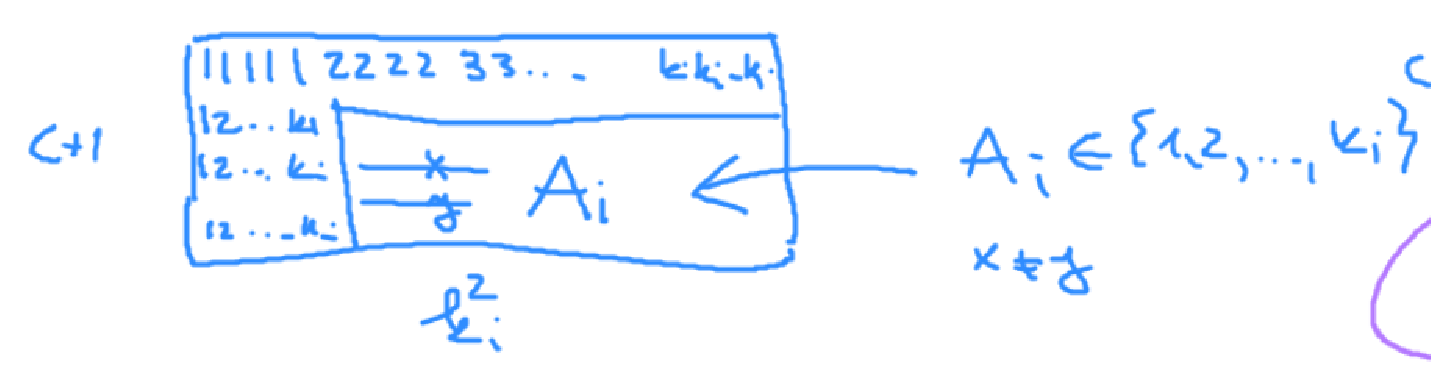
\includegraphics[scale=0.5]{lc_2.eps}

	Zafixujme nyní $(v, k_1, k_2, \ldots, k_r; k_{r + 1}, \ldots, k_m, 1)$-BIBD $(V, \B)$, který podle předpokladu existuje, a nechť $S_1, S_2, \ldots, S_b$ jsou bloky.
	Pro každý blok $S_j$ velikosti $k_i$ vytvoříme matici $B_j$ z matice $A_i$ tak, že symboly $1, 2, \ldots, k_i$ nahradíme jmény prvků z bloku $S_j$.
	Potom matice
	\[ (B_1, \ldots, B_b, E) \]
	kde $E$ je matice obsahující sloupce $(x, \ldots, x)^T$ pro všechna
	\[ x \in V \setminus \{ \bigcup_{S_j \in \bigcup_i^r \B_i} S_j \]
	Pak tato matice je matice OA($v, c$) $\stackrel{\cref{nolc_oa}}{\Rightarrow} NOLČ(v) \geq c - 2$.
\end{proof}

\begin{example}
	KPR(4) = $(21, 5, 1)$-BIBD $\stackrel{\cref{nolc_lower_2}}{\Rightarrow}NOLČ(21) \geq NOLČ(5) - 1 = 3$.

	To je protipříklad na hypotézu McNeishe $NOLČ(p_i^{r_i}) = \min_i \{ p_i^{r_i} - 1 \}$.
\end{example}

\begin{theorem}[$(v,k,1)$-BIBD a NOLČ]
    Existuje-li $(v,k,1)$-BIBD, pak
    \begin{itemize}
        \item[1)] NOLČ($v-1$)$\geq\min($NOLČ$(k-1),$NOLČ$(k)-1)$
        \item[2)] Pro $2\leq x\leq k$, pak NOLČ$(v-x)\geq\min\{$NOLČ$(k-x),$NOLČ$(k)-1,$NOLČ$(k-1)-1\}$
    \end{itemize}
\end{theorem}
\begin{proof}
    \begin{itemize}
        \item[1)]  Z blokového schématu $(v, k, 1)$-BIBDu zahoďme jeden prvek.
		Dostaneme tak $(v-1, k - 1; k, 1)$-BIBD (protože $r - 1$ bloků o $k - 1$ prvcích je po dvou disjunktních).

		\[ (V, \B) \to (V \setminus \{ a \}, \B^{\prime}) \]
		% todo obrazek

        \item[2)] Z blokového schématu $(v, k, 1)$-BIBD zahoďme $x$ prvků, které patří do stejného bloku.
		Dostaneme tak $(v - x, k - x; k - 1, k, 1)$-BIBD (protože jediný blok o $k - x$ prvcích triviálně tvoří průhlednou množinu).

    \end{itemize}
\end{proof}

\begin{theorem}[$(v,k,1)$-BIBD a NOLČ($v-3$)]\label{nolc_lower_3}
    Existuje-li $(v,k,1$)-BIBD, pak NOLČ($v-3$)$\geq\min\{$NOLČ($k-2$),NOLČ($k-1)-1$,NOLČ($k$)$-1\}$.
\end{theorem}
\begin{proof}
	Z blokového schématu (v, k, 1)-BIBD zahoďme tři prvky, které neleží ve stejném bloku.
	Dostaneme tak $(v - 3, k - 2; k, k - 1, 1)$-BIBD (protože bloky o $k - 2$ prvcích jsou po dvou disjunktní).

	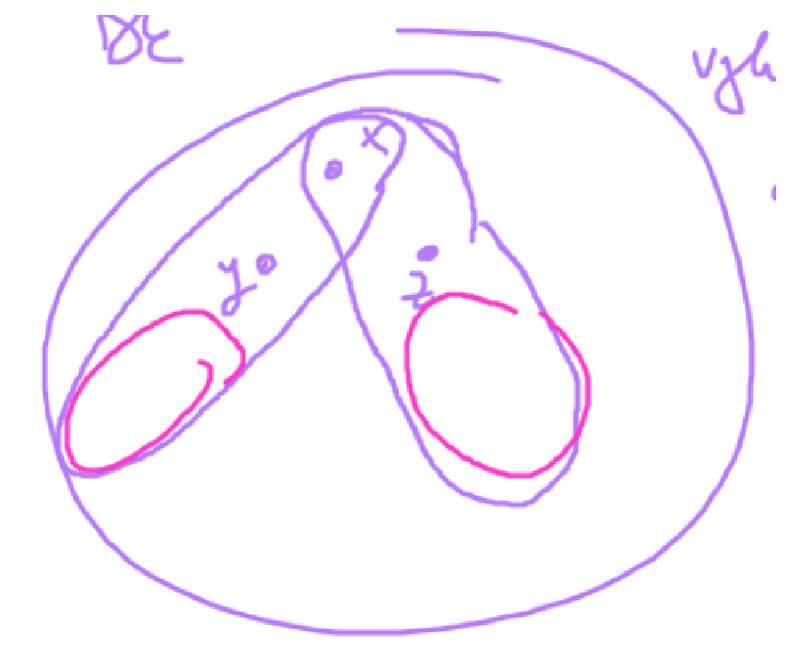
\includegraphics[scale=0.4]{lc_3.eps}
\end{proof}

\begin{example}
	KPR(4) = $(21, 5, 1)$-BIBD $\stackrel{\cref{nolc_lower_3}}{\Rightarrow}$:
	\[ NOLČ(18) \geq \min \{ NOLČ(3) = 2, NOLČ(5) - 1 = 3, NOLČ(4) - 1 = 2 \} = 2 \]

	Přitom $18 \equiv 2 mod 4$, ale 18 není tvaru $12k + 10$.
\end{example}

\begin{definition}[Řešitelný systém]
	%todo why sqcup? disjoint union?
    Systém $(V,\mathcal{B})$ je řešitelný, pokud $\mathcal{B}=\mathcal{B}1\sqcup\ldots\sqcup\mathcal{B}_r$ takový, že
    \begin{enumerate}
        \item $\forall i: \mathcal{B}_i$ je průhledná
        \item $\bigcup\mathcal{B}_i=B$
    \end{enumerate}

    Pak $\mathcal{B}_i$ nazveme třídy řešitelnosti.
\end{definition}

\begin{example}[Řešitelný systém]
	Každá KAR řádu $m$ je řešitelný $(m^2, m, 1)$-BIBD s $(m + 1)$ třídami řešitelnosti.

	% todo popis
	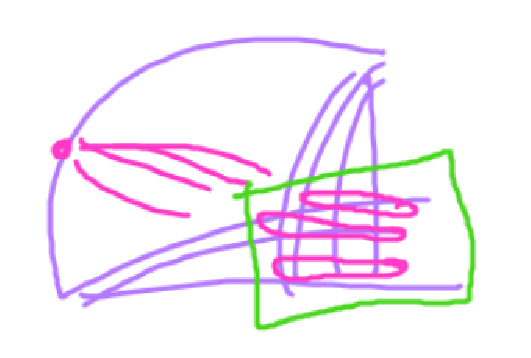
\includegraphics[scale=0.4]{lc_4.eps}
\end{example}

\begin{theorem}[Řešitelnost a odhady na NOLČ]
    Pokud existuje řešitelný $(v,k,1)$-BIBD a r třídami řešitelnosti, pak
    \begin{enumerate}
        \item NOLČ($v+1$)$\geq\min\{$NOLČ($k$)$-1$, NOLČ($k+1$)$-1\}$
        \item pro $2\leq x\leq r-2:$ NOLČ($v+x$)$\geq\min\{$NOLČ($x$),NOLČ($k$)$-1$, NOLČ($k+1$)$-1\}$
        \item NOLČ($v+r-1$)$\geq\min\{$NOLČ($r-1$),NOLČ($k$), NOLČ($k+1$)$-1\}$
        \item NOLČ($v+r$)$\geq\min\{$NOLČ($r$), NOLČ($k+1$)$-1\}$
    \end{enumerate}
\end{theorem}
\begin{proof}
    TODO
\end{proof}

\begin{example}[Řešitelný systém 2]
	TODO whiteboard
\end{example}

\begin{definition}[Skupinově rozložitelný systém]
    Množinový systém $(V,\mathcal{B})$ se nazývá skupinově rozložitelný (group divisible), pokud $\exists V_1,\ldots, V_n: V_i\subseteq V, V_i\cap V_j=\emptyset$.
    \begin{itemize}
        \item[a)] $\forall x,y\in V_i: \exists \lambda_1$ bloků sdílejících $x,y$
        \item[b)] pro $i\neq j$: $\forall x\in V_i, \forall y\in V_j: \exists\lambda_2$ bloků sdílejících $x,y$.
    \end{itemize}
    Pokud všechny bloky mají velikost $k$, $|V_i|=m$, pak značíme systém jako $GD(v,k,m,\lambda_1,\lambda_2)$.

	Často se říká, že \# skupin je $n \Rightarrow v = n m$.
\end{definition}
\begin{theorem}[NOLČ a existence GD]
    Pokud pro $m,k$ platí NOLČ($m$)$\geq k-1$, pak $\exists GD(km,k,m,0,1)$ s $m$ třídami řešitelnosti.
\end{theorem}
\begin{proof}
	NOLČ($m$)$\geq k-1 \Rightarrow \exists OA(m, k + 1)$.
	BUNO poslední řádek v tabulce má symbol $i$ v $i$-tem bloku.
	Tento řádek zahodíme.

	Prvek na pozice $(i, j)$ nahradíme právě dvojici souřadnic, takže stejná písmena v různých řádcích jsou odlišné.
	Postavíme množinový systém:
	\[ V = \{ 1, \ldots, k \} \times \{ 1, \ldots, n \} \]
	kde $1 - k$ jsou původní symboly a $1 - n$ jsou "barvy".

	% predn 8 17:20
	\begin{figure}
	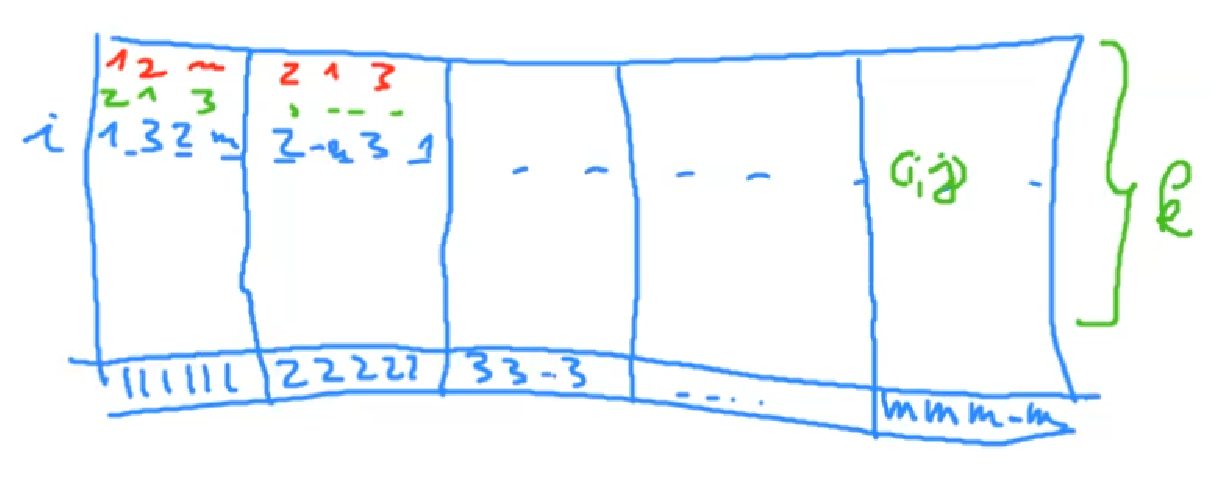
\includegraphics[scale=0.4]{lc_5.eps}
	\caption{\small \sl GD NOLČ
	\label{fig:nolc_gd_obr}}
	\end{figure}

	Řádky OA tvoří třídy řešitelnosti velikosti $m$, bloky jsou sloupce OA (bereme jeden prvek každé barvy).

	% predn 8 18:00
	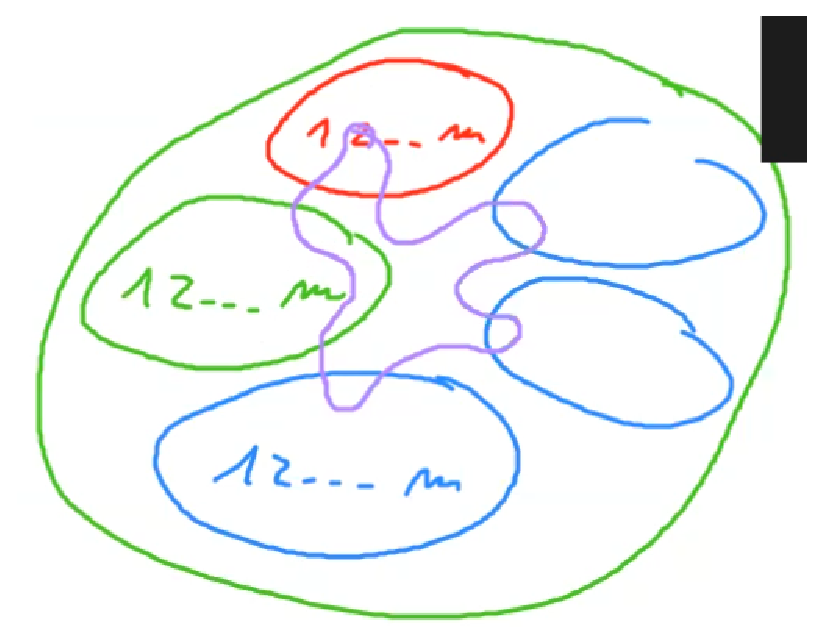
\includegraphics[scale=0.4]{lc_6.eps}

	Z konstrukce máme parametry $GD(km,k,m, ?, ?)$, zbývá zkontrolovat $\lambda_1, \lambda_2$.
	Nechť $x, y$ jsou libovolné 2 prvky ze stejné skupiny nějaké barvy.
	Jelikož do bloku vždy bereme jenom 1 prvek z barevné skupiny, nemůžou být ve stejném bloku $\Rightarrow GD(km,k,m, 0, ?)$.

	Nechť $x, y$ jsou libovolné prvky z dvou skupin různých barev.
	Z vlastnosti OA symboly $x, y$ jsou nad sebou pravě v jediném sloupci $\Rightarrow GD(km,k,m, 0, 1)$.

	Konečně zkontrolujeme řešitelnost.
	Každý obdélník na obrázku \cref{fig:nolc_gd_obr} tvoří průhlednou množinu.
	Všechny takové pokrývají celý systém.
\end{proof}
\begin{theorem}[Řešitelný GD a NOLČ]
    Existuje-li $GD(v,k,m,0,1)$ řešitelný, GD má $r$ tříd řešitelnosti, pak
    \[\forall x \in [r - 1]: NOLČ(v+x) \geq \min \{NOLČ(m), NOLČ(x), NOLČ(k)-1, NOLČ(k+1)-1\} \]
\end{theorem}
\begin{proof}
	Označme skupiny rozložitelnosti $V_1, \ldots, V_n$, pak $v = mn$.
	Přidáme skupiny jako bloky
	\[ (V, \B) \to (V, \B^{\prime}), \B^{\prime} = \B \cup \{ V_1, \ldots, V_n \} \]
	Pak $(V, \B^{\prime})$ je $(v, m; k, \lambda = 1)$-BIBD.
	$\lambda$ je uniformní, protože prvky z $S_i$ teď patří do 1 společného bloku.
	Navíc bloky $S_i$ velikosti $m$ jsou po 2 disjunktní.
	Pozor, toto neplatí pro $m = k$, tady průhlednou množinu tvoří právě bloky $V_1, \ldots, V_n$.

	Přidáme navíc prvky $y_1, \ldots, y_x$, taky přidáme blok $\{ y_1, \ldots, y_x \}$.
	Do všech množin z $i$-te třídy řešitelnosti přidáme prvek $y_i$.
	Čímž vznikne množinový systém $(V^{\prime}, \B^{\prime\prime})$.
	Kde $|V^{\prime}| = v + x$ a je to $(v + x, m, k + 1, k, ?, ?)$.

	% predn 8 39:00
	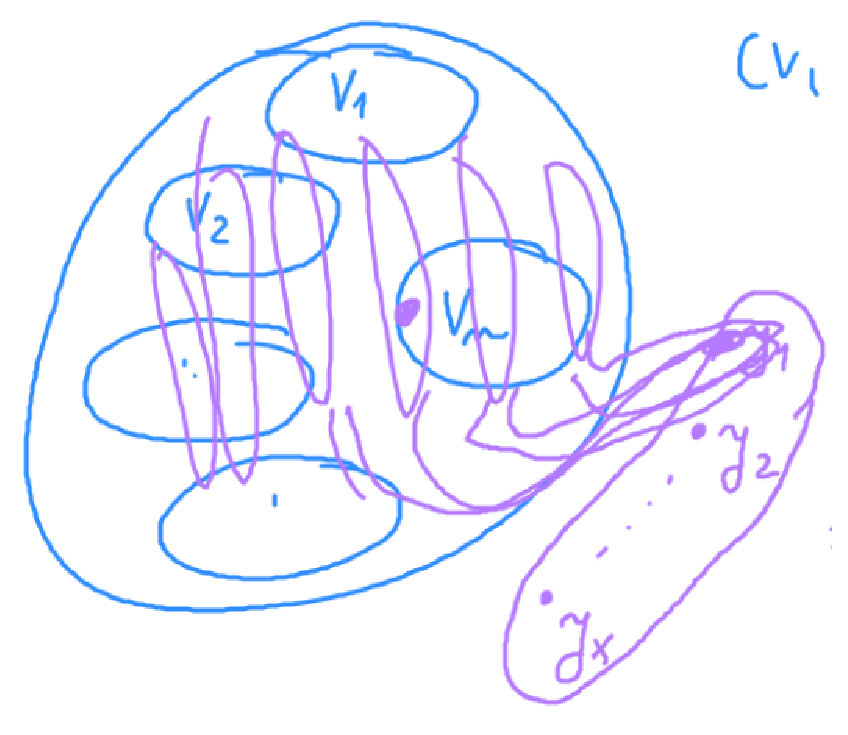
\includegraphics[scale=0.4]{lc_7.eps}

	Zkontrolujeme $\lambda$ rozborem případu:
	\begin{itemize}
		\item 2 prvky z modrých množin pořad jsou v 1 společném bloku.
		\item prvek $y_i$ a nějaký prvek z třídy řešitelnosti je právě v 1 bloku
		\item 2 prvky $y_i, y_k$ jsou v 1 nově přidaném bloku.
	\end{itemize}
	Dohromady máme $(v + x, m, x; k + 1, k, \lambda = 1)$-BIBD.
	Navíc bloky tvořící skupiny rozložitelnosti a nový blok $y$-nů tvoří průhlednou množinu.
	Dle \cref{nolc_lower_2}:
	\[ NOLČ(v+x) \geq \min \{NOLČ(m), NOLČ(x), NOLČ(k)-1, NOLČ(k+1)-1\} \]

	Když $m = k$ tak $NOLČ(m)$ je v $\min$ zbytečný, protože $NOLČ(k)-1$ je o 1 menší.
	Neboli v tomto případě nezáleží jestli bloky skupiny řešitelnosti tvoří průhlednou množinu.

	Taky ale může být $m = k + 1, x = k, x = k + 1$.
	Všechny tyto případy jsou analogické $m = k$.
\end{proof}

\begin{consequence}[O násobení NOLČ]\label{nolc_mult}
    Je-li NOLČ($m$)$\geq k-1$, pak
    \[ \forall x \in [r-1]: NOLČ(km+x) \geq \min\{NOLČ(m), NOLČ(x), NOLČ(k)-1, NOLČ(k+1)-1\} \]
    Ale kvůli tomu, že třídy řešitelnosti jsou obdélníky na obrázku \cref{fig:nolc_gd_obr} a jsou velikosti $m$ můžeme vzít vetší $x$:
    \[ \forall x \in [m-1]: NOLČ(km+x) \geq \min\{NOLČ(m), NOLČ(x), NOLČ(k)-1, NOLČ(k+1)-1\} \]
\end{consequence}
%\begin{proof}
%    TODO
%\end{proof}

\begin{lemma}[Dolni odhad pro NOLČ]\label{nolc_lower_4}
    Pokd NOLČ$(4t+2) \geq 2$ pro každé $2\leq t\leq 181$, pak NOLČ($4t+2$)$\geq 2$ pro každé $t\geq 2$.

    Znění říká, že pokud existuji aspoň 2 ortogonální LČ pro $10, 14, 18, \ldots, 5 \cdot 181 +2 = 726$.
\end{lemma}
\begin{proof}
	Nechť $t \geq 730, v = 4t + 2$.
	Podělíme $v - 10$ číslem 144: $v - 10 = 144 g + z, z \in [0, 144)$.
	Jelikož $v, 10 \equiv 2 \mod4$ tak jejich součet je dělitelný 4.
	Taky $144 = 36 \Rightarrow z = 4u, u \in [0, 36)$.

	Přepíšeme $v = 4 \cdot 36g + 4u + 10$.
	Dal
	\[ NOLČ(36g) = NOLČ(2^{\geq 2} \cdot 3^{\geq 2} \cdot 5 \cdot \ldots) \geq \min(NOLČ(2^{\geq 2}), NOLČ(3^{\geq 2}), \ldots) \stackrel{\cref{nolc_lower_0}}{\geq} \min(3, 8, \geq 3, \ldots) = 3 \geq k - 1 \]
	Použijeme \cref{nolc_mult} s $m = 36g, k = 4, x = 4u + 10$.
	\begin{gather*}
		NOLČ(m) \geq k - 1 \stackrel{\cref{nolc_mult}}{\Rightarrow} NOLČ(mk + x) = NOLČ(v) \geq \\
		\geq \min(NOLČ(36g) \geq 3, NOLČ(4u + 10), NOLČ(4) - 1 = 2, NOLČ(5) - 1 = 3) \\
	\end{gather*}
	Taky $10 \leq 4u + 10 \leq 4\cdot35 + 10 = 150 \leq 726$.
	Takže dle předpokladu $NOLČ(4u + 10) \geq 2$.
	Neboli
	\[ \min(NOLČ(36g) \geq 3, NOLČ(4u + 10) \geq 2, NOLČ(4) - 1 = 2, NOLČ(5) - 1 = 3) = 2 \]
\end{proof}

\begin{theorem}[NOLČ je aspoň 2]
    $\forall v>6:$ NOLČ($v$)$\geq 2$.
\end{theorem}
\begin{proof}
	Pokud $v \not\equiv 2 \mod4$ tak jsme dokázali v \cref{nolc_lower_1}.

	Jinak $v \equiv 2 \mod4 \& v \leq 726$ věříme jako fakt.
	Pro $v \geq 730$ existuje z \cref{nolc_lower_4}.
\end{proof}
